\documentclass{standalone}
\usepackage{amssymb}
\usepackage{tikz}
\usetikzlibrary{matrix,arrows.meta,calc,positioning,trees,fit}

\pgfdeclarelayer{background}
\pgfdeclarelayer{foreground}
\pgfsetlayers{background,main,foreground}

\begin{document}
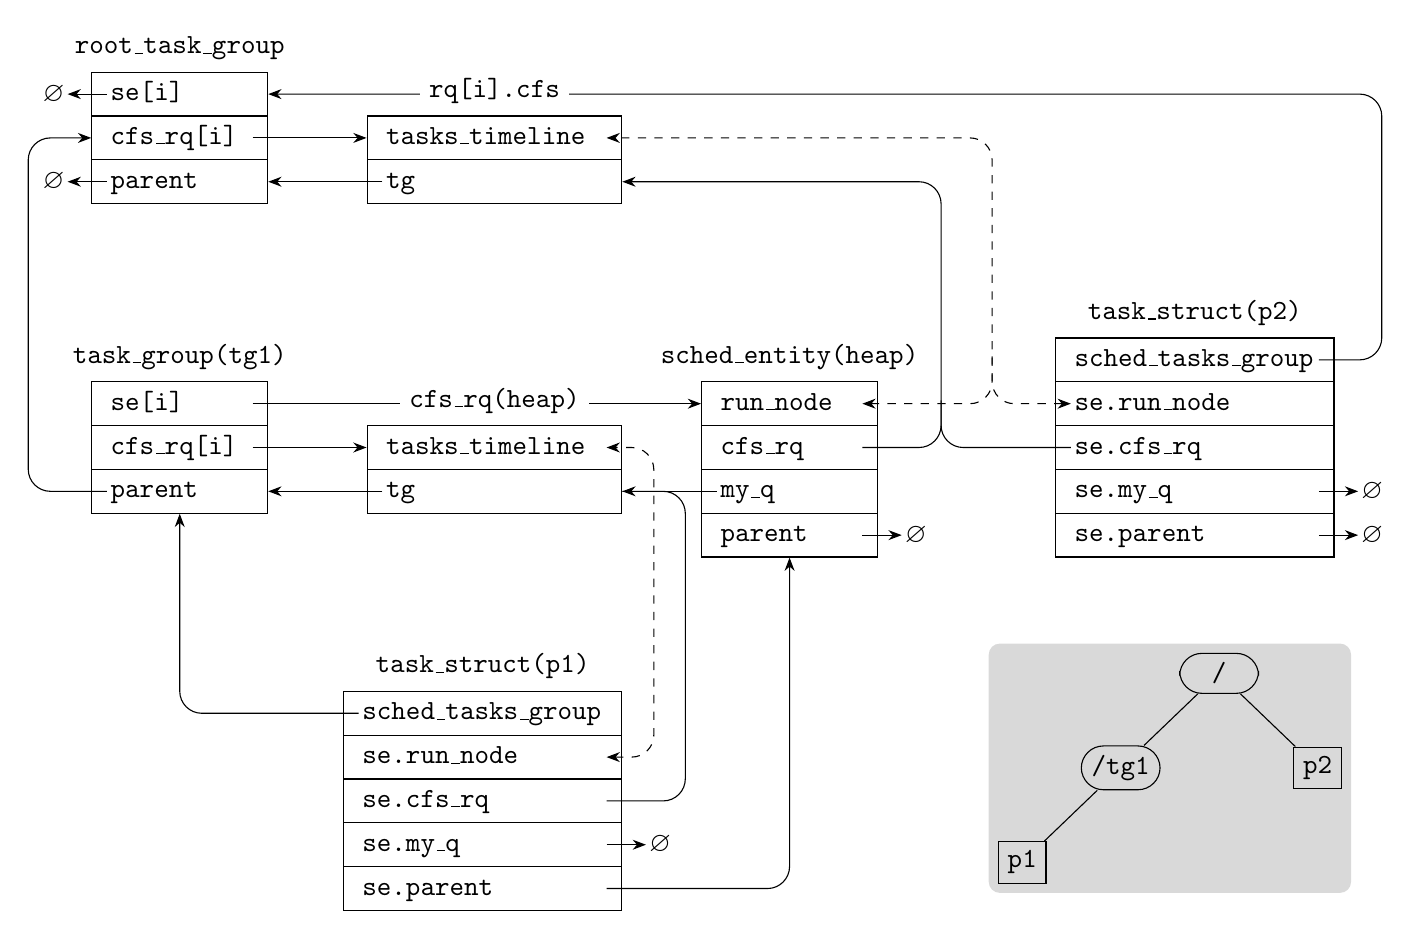
\begin{tikzpicture}
  [
    font = \ttfamily,
    every node/.style = {
      draw,
    },
    every label/.style = {
      draw = none,
      fill = white,
    },
    label distance = -1mm,
    nil/.style = {
      draw = none,
      inner sep = 1pt,
    },
    > = Stealth,
    sibling distance = 2.5cm,
    level distance = 1.2cm,
  ]

  \matrix (roottg) [
    draw = none,
    matrix of nodes,
    text width = 2cm,
    row sep = -\pgflinewidth,
    label = above:root\_task\_group,
  ]{
    \vphantom{p[} se[i]      \\
    \vphantom{p[} cfs\_rq[i] \\
    \vphantom{p[} parent     \\
  };

  \matrix (rootcfs) [
    draw = none,
    matrix of nodes,
    text width = 3cm,
    row sep = -\pgflinewidth,
    label = above:{rq[i].cfs},
    right = of roottg.south east,
    anchor = south west,
  ]{
    \vphantom{p[} tasks\_timeline \\
    \vphantom{p[} tg              \\
  };

  \matrix (tg1) [
    draw = none,
    matrix of nodes,
    text width = 2cm,
    row sep = -\pgflinewidth,
    label = above:task\_group(tg1),
    below = 20mm of roottg,
  ]{
    \vphantom{p[} se[i]      \\
    \vphantom{p[} cfs\_rq[i] \\
    \vphantom{p[} parent     \\
  };

  \matrix (cfs1) [
    draw = none,
    matrix of nodes,
    text width = 3cm,
    row sep = -\pgflinewidth,
    label = above:cfs\_rq(heap),
    right = of tg1.south east,
    anchor = south west,
  ]{
    \vphantom{p[} tasks\_timeline \\
    \vphantom{p[} tg              \\
  };

  \matrix (se1) [
    draw = none,
    matrix of nodes,
    text width = 2cm,
    row sep = -\pgflinewidth,
    label = above:sched\_entity(heap),
    right = of cfs1-2-1,
    anchor = se1-3-1.west,
  ]{
    \vphantom{p[} run\_node \\
    \vphantom{p[} cfs\_rq   \\
    \vphantom{p[} my\_q     \\
    \vphantom{p[} parent    \\
  };

  \matrix (task1) [
    draw = none,
    matrix of nodes,
    text width = 3.3cm,
    row sep = -\pgflinewidth,
    label = above:task\_struct(p1),
    below = 20mm of cfs1.south east,
    anchor = north east,
  ]{
    \vphantom{p[} sched\_tasks\_group \\
    \vphantom{p[} se.run\_node        \\
    \vphantom{p[} se.cfs\_rq          \\
    \vphantom{p[} se.my\_q            \\
    \vphantom{p[} se.parent           \\
  };

  \matrix (task2) [
    draw = none,
    matrix of nodes,
    text width = 3.3cm,
    row sep = -\pgflinewidth,
    label = above:task\_struct(p2),
    right = 20mm of se1.south east,
    anchor = south west,
  ]{
    \vphantom{p[} sched\_tasks\_group \\
    \vphantom{p[} se.run\_node        \\
    \vphantom{p[} se.cfs\_rq          \\
    \vphantom{p[} se.my\_q            \\
    \vphantom{p[} se.parent           \\
  };

  \begin{pgfonlayer}{background}
    \draw [->] ([xshift=2mm] roottg-1-1.west) -- +(-5mm, 0) node[nil,anchor=east]{$\varnothing$};
    \draw [->] ([xshift=2mm] roottg-3-1.west) -- +(-5mm, 0) node[nil,anchor=east]{$\varnothing$};
    \draw [->] ([xshift=-2mm] se1-4-1.east) -- +(5mm, 0) node[nil,anchor=west]{$\varnothing$};
    \draw [->] ([xshift=-2mm] task1-4-1.east) -- +(5mm, 0) node[nil,anchor=west]{$\varnothing$};
    \draw [->] ([xshift=-2mm] task2-4-1.east) -- +(5mm, 0) node[nil,anchor=west]{$\varnothing$};
    \draw [->] ([xshift=-2mm] task2-5-1.east) -- +(5mm, 0) node[nil,anchor=west]{$\varnothing$};

    \draw [->] ([xshift=-2mm] roottg-2-1.east) -- (rootcfs-1-1);
    \draw [->] ([xshift=2mm] rootcfs-2-1.west) -- (roottg-3-1);

    \draw [->] ([xshift=-2mm] tg1-1-1.east) -- (se1-1-1);
    \draw [->] ([xshift=-2mm] tg1-2-1.east) -- (cfs1-1-1);
    \draw [->,rounded corners=8pt] ([xshift=2mm] tg1-3-1.west) -- +(-10mm,0) |- (roottg-2-1.west);

    \draw [->] ([xshift=2mm] cfs1-2-1.west) -- (tg1-3-1);

    \coordinate (tree merge) at ($ (task2-2-1.west) + (-8mm, 0) $);
    \coordinate (cfs merge) at ($ (se1-2-1.east) + (8mm, 0) $);

    \draw [->] ([xshift=2mm] se1-3-1.west) -- (cfs1-2-1);
    \draw [<->,dashed,rounded corners=8pt] ([xshift=-2mm] se1-1-1.east) -- (tree merge) |- ([xshift=-2mm] rootcfs-1-1.east);
    \draw [->,rounded corners=8pt] ([xshift=-2mm] se1-2-1.east) -- (cfs merge) |- (rootcfs-2-1.east);

    \draw [->,rounded corners=8pt] ([xshift=-2mm] task2-1-1.east) -- +(8mm,0) |- (roottg-1-1.east);
    \draw [<-,dashed,rounded corners=8pt] ([xshift=2mm] task2-2-1.west) -- (tree merge) -- +(0, 6mm);
    \draw [rounded corners=8pt] ([xshift=2mm] task2-3-1.west) -- (cfs merge) -- +(0, 6mm);

    \draw [->,rounded corners=8pt] ([xshift=2mm] task1-1-1.west) -| (tg1-3-1.south);
    \draw [<->,dashed,rounded corners=8pt] ([xshift=-2mm] task1-2-1.east) -- +(6mm, 0) |- ([xshift=-2mm] cfs1-1-1.east);
    \draw [rounded corners=8pt] ([xshift=-2mm] task1-3-1.east) -- +(10mm, 0) |- (cfs1-2-1.east);
    \draw [->,rounded corners=8pt] ([xshift=-2mm] task1-5-1.east) -| (se1-4-1.south);
  \end{pgfonlayer}

  \node (a) [
    rounded corners = 8pt,
    minimum width = 1cm,
  ] at (13.2cm, -6.8cm) {/}
    child {node (b) [rounded corners=8pt,minimum width=1cm] {/tg1}
      child {node (c) {p1}}
      child [ missing ]
    }
    child {node (d) {p2}};
  \begin{pgfonlayer}{background}
    \node [
      draw = none,
      rounded corners,
      fill = black!15,
      fit=(a)(b)(c)(d),
    ] {};
  \end{pgfonlayer}

\end{tikzpicture}
\end{document}
